% `template.tex', a bare-bones example employing the AIAA class.


\documentclass[]{aiaa-tc}% insert '[draft]' option to show overfull boxes
\usepackage{amsmath}
\usepackage{SIunits}
\usepackage{xcolor}

 %\title{High enthalpy effects on hypersonic boundary-layer transition}
 \title{Code to code comparison on hypersonic high enthalpy transitional boundary layers}


\author{
  Viola Wartemann%
   \thanks{Research Scientist, Spacecraft Department, DLR Braunschweig, Viola.Wartemann@dlr.de}\\
  {\normalsize\itshape
  German Aerospace Center (DLR), Institute of Aerodynamics and Flow Technology, Braunschweig, Germany} \\
  \and
  Ross Wagnild%
    \thanks{Research Scientist, Sandia National Laboratories, Albuquerque, USA, rmwagni@sandia.gov} \\
{\normalsize\itshape
  Sandia National Laboratories, Albuquerque, USA} \\
  \and
  Fabio Pinna%
    \thanks{Research Scientist, von Karman Institute for Fluid Dynamics, Rhode-St-Genèse, Belgium, fabio.pinna@vki.ac.be} \\
{\normalsize\itshape
  von Karman Institute for Fluid Dynamics, Aeronautics and Aerospace Department, Rhode-St-Genèse, Belgium} \\
    \and
  Fernando Miro%
    \thanks{PhD Student, von Karman Institute for Fluid Dynamics, Rhode-St-Genèse, Belgium, fernando.miro.miro@vki.ac.be} \\
{\normalsize\itshape
  von Karman Institute for Fluid Dynamics, Aeronautics and Aerospace Department, Rhode-St-Genèse, Belgium} \\
  \and
  Hideyuki Tanno% 
    \thanks{Research Scientist, Japan Aerospace Exploration Agency, Kimigaya, Japan, tanno@spaceships.isas.jaxa.jp} \\
{\normalsize\itshape
 Japan Aerospace Exploration Agency, Kimigaya, Japan} \\
  Alexander Wagner% 
   \thanks{Research Scientist, Spacecraft Department, DLR G\"ottingen, Alexander.Wagner@dlr.de} \\
  {\normalsize\itshape
  German Aerospace Center (DLR), Institute of Aerodynamics and Flow Technology, G\"ottingen, Germany} \\
}

 % Data used by 'handcarry' option if invoked
 \AIAApapernumber{YEAR-NUMBER}
 \AIAAconference{Conference Name, Date, and Location}
 \AIAAcopyright{\AIAAcopyrightD{YEAR}}

 % Define commands to assure consistent treatment throughout document
 \newcommand{\eqnref}[1]{(\ref{#1})}
 \newcommand{\class}[1]{\texttt{#1}}
 \newcommand{\package}[1]{\texttt{#1}}
 \newcommand{\file}[1]{\texttt{#1}}
 \newcommand{\BibTeX}{\textsc{Bib}\TeX}

\begin{document}

\maketitle


\begin{abstract}

\textcolor{red}{Till now: it is just the abstract with some comments from me and some additional headings. \\ red color: comments for all}\\
\textcolor{blue}{comments for Ross}\\
\textcolor{green}{comments for Fabio and Fernando}\\
\textcolor{cyan}{comments for Tanno}\\
\textcolor{magenta}{comments for Alex}

In the scope of the present study three hypersonic stability codes are compared based on hypersonic high enthalpy boundary layer flow around a $\unit{7}{\degree}$ blunted cone. The code to code comparison is conducted between the following codes: the  NOnLocal Transition analysis code (NOLOT) of the German Aerospace Center (DLR), the Stability and Transition Analysis for hypersonic Boundary Layers code (STABL) of University of Minnesota and the VKI Extensible Stability and Transition Analysis code (VESTA) of the von Karman Institute. The comparison will focus on the role of real gas effects on the second mode instability, in particular its frequency and growth rate. The experimental test cases for the code to code comparison are provided by the DLR High Enthalpy Shock Tunnel G\"ottingen (HEG) and the JAXA shock tunnel HIEST.  

\end{abstract}


\section*{Abbreviations}
\begin{tabular}{lll}
DLR   &    &  German Aerospace Center \\
JAXA & &  Japan Aerospace Exploration Agency\\
NOLOT & & NOnLocal Transition analysis code\\
STABL & & Stability and Transition Analysis for hypersonic Boundary Layers\\
VESTA & & VKI Extensible Stability and Transition Analysis toolkit \\
VKI & &  von Karman Institute for Fluid Dynamics\\

\end{tabular}

\section{Introduction}

Laminar to turbulent transition in high-speed boundary-layers is of high importance for re-entry vehicles since early transition results in an increase in the heat transfer by factors between 3 and 8, resulting in a cost and weight increase of thermal protection systems \cite{Schneider_1999,Schneider_2004}. The second mode instability, commonly referred as Mack mode \cite{Mack_1984}, is the dominant mode for essentially 2D boundary layers at high local Mach number ($M\hspace{-0.08cm} a_e > 4$) and/or cold walls\cite{Mack_1984}. Thus the second mode is in the main focus of the investigations of this paper. High speed vehicles and re-entry vehicles operate in an high enthalpy range. In this range real gas effect occurs, which can include molecular rotation, molecular vibration, chemical dissociation and exchange, electronic excitation, radiation and ionization. In this paper the high enthalpy effects on the second modes are investigated. The numerical investigations are performed with three different stability codes, which are compared against each other: the NOLOT code of the DLR, the STABL code from the University of Minnesota and the VESTA code of VKI. The base flow as well as the stability calculations itself are performed with and without real gas effects for the comparison.\\

Further the stability results are compared against low and high enthalpy experiments, which were performed on a blunted $7^\circ$ half-angle cone model. Two of the chosen experiments for the comparison were performed in the DLR High Enthalpy Shock Tunnel G\"ottingen (HEG) and one additional experiment was performed in the JAXA High Enthalpy Shock Tunnel (HIEST).


\section{Numeric methods}
The equations of the stability codes are derived from the conservation equations of mass, momentum and energy, which govern the flow of a viscous, compressible gas. All flow and material quantities are decomposed into a steady laminar base flow $\bar{q}$ and an unsteady 
disturbance flow $\tilde{q}$\
\begin{equation}
q(x,y,z,t)=\bar{q}(x,y)+\tilde{q}(x,y,z,t).
\end{equation}
The  laminar base-flow $\bar{q}$ are calculated by different CFD codes, which solves the Navier-Stokes equations, and can be used without and with chemistry. The disturbance $\tilde{q}$ is represented as a harmonic wave
\begin{equation}
\tilde{q}(x,y,z,t)=\hat{q}(x,y)\exp[i(\alpha x + \beta z - \omega t)]\label{wave}
\end{equation}
with the complex-valued amplitude function $\hat{q}$. \\

All codes can be used for Linear Stability Theory (LST) as well as Parabolized Stability Equations (PSE) analyses. In contrast to STABL and VESTA, which can exclude or include chemistry, NOLOT is limited on the perfect gas assumption.  

\subsection{STABL}
\textcolor{blue}{It make sense to describe one code in more detail and not all codes. The STABL code is the code with the most options (especially, the chemistry option), thus I would suggest to describe the STABL code in more detail. Please, add a description of your stability code.}
\subsection{VESTA}
\textcolor{green}{Please, add a short description of your stability code.}
\subsection{NOLOT}

\section{Wind tunnels and wind tunnel model}\label{sect:model}
For both wind tunnels a similar, not the same, cone model is used: a $7^\circ$ half-angle blunted cone with an overall length of about $1 \hspace{0.05cm} \rm m$ and an nose tip radius of $2.5\hspace{0.05cm} \rm mm$ (see picture \ref{fig:cone_model}). Both models were equipped with thermocouples and pressure transducers. The models were supported by a sting system at nominal $0^\circ$ angle of attack.\\

\begin{figure}[htbp]
	\centering
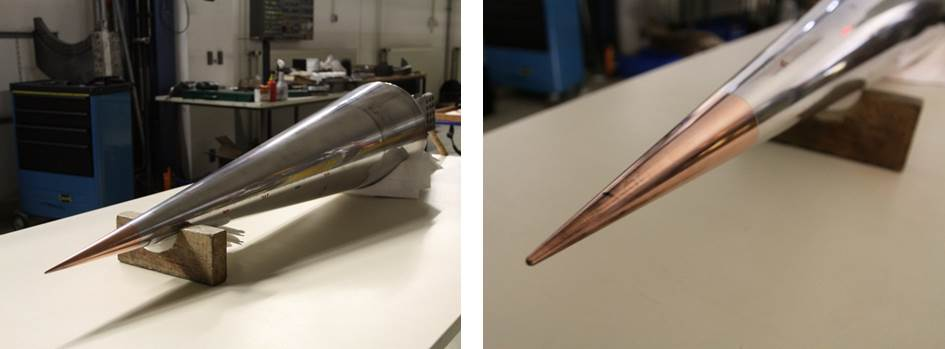
\includegraphics[width=0.8\textwidth]{pics/2018_cone_model.jpg}
	\caption{JAXA $\unit{7}{\degree}$ cone model.}
	\label{fig:cone_model}
\end{figure}

Two of the chosen experiments for the comparison with the numerical codes were performed in the HEG. The tunnel is a free piston driven shock tunnel, which allows to investigate flow past hypersonic flight configurations from low altitude Mach 6 up to Mach 10 at approximately $33 \hspace{0.05cm} \rm km$ altitude. In this operating range, total specific enthalpies of up to 22 MJ/kg can be reached.\cite{Hannemann_2008} The two investigated HEG experiments in this paper have a unit Reynolds numbers of $Re_{\rm m} = 1.4 \times 10^6 / \rm m$ at different enthalpies (see table \ref{tab:test_cases}). As reference case, one experiment with low enthalpy (HEG-Low-E) is chosen. The second selected HEG experiment is with high enthalpy (HEG-High-E). Additionally, a high enthalpy experiment, performed by JAXA in HIEST (HIEST-High-E), which is in a comparable range of the high enthalpy test case of HEG, is selected for the numerical analyses.

\textcolor{cyan}{The focus in the paper is the numerical comparison, thus the description of the wind tunnels is very short. Please, feel free to add some sentences.}\\
\textcolor{magenta}{same comment for you Alex}

\begin{table}[htbp]
	\centering
\begin{tabular}{c||c|c|c|c|c|c|c|c|c}%
 Test Case & $p_{\infty} [Pa] $&  $T_{\infty} [K] $  & $\rho_{\infty} [kg/m^3] $ & $u_{\infty} [m/s]$ & $M\hspace{-0.08cm}a_{\infty}$ & $T_w [K] $ & $Re_{\rm m} [10^6/m$ & $h_0 [MJ/kg]$ \\
\hline
\hline
\hspace{0.15cm} HEG-Low-E& \hspace{0.08cm} 816 & \hspace{0.08cm} 264 & 0.0107 &  2399 & 7.35   & 293 & 1.55 &\hspace{0.08cm} 3.1\\
\hline
\hspace{0.15cm} HEG-High-E& 6578  & 1286  & 0.0171 &  4354 &  6.09      & 293 & 1.52 & 11.6\\
\hline
HIEST-High-E&   &   &      & &  & & & \\
\end{tabular}
	\caption{Operating conditions of the presented study}
	\label{tab:test_cases}
\end{table}

\textcolor{red}{Thanks Tanno for your data. Alex selected one test case, which is in a comparable range to the HEG high enthalpy case. I will send the free stream condition in an additional email.}

\section{Results}\label{sect:results}

\subsection{Low enthalpy test case (HEG)}\label{sect:low_enthalpy}

\subsubsection{LST comparison (VESTA / NOLOT)}
\subsubsection{PSE comparison (STABL / NOLOT)}
\subsubsection{Comparison with the HEG experiment}

\subsection{First high enthalpy test case (HEG)}\label{sect:high_enthalpy}

\subsection{Second high enthalpy test case (HIEST)}\label{sect:high_enthalpy}

\textcolor{red}{the rest is just old stuff from the abstract, which I will replace soon}
This section summarized the first results of the numerical comparison. In figure \ref{fig:1324_n_x} the N-factors of the second mode calculated by NOLOT as a function of the normalized $x$-position are shown for different frequencies. Out of this diagram the N-factors can be extracted from sensor positions of the experiment for various frequencies, which is visible in figure \ref{fig:1324_n_f} for the three pressure sensor positions of the HEG-High-E experiments. 

\begin{figure}[htbp]
	\centering
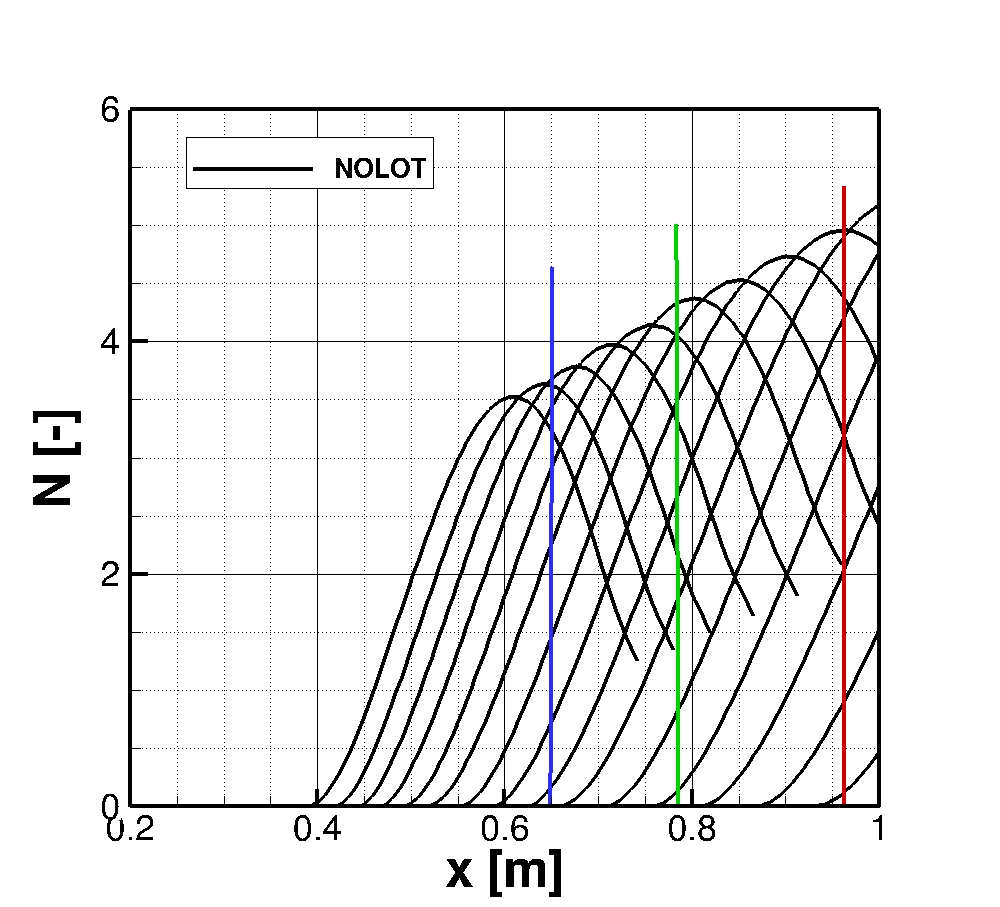
\includegraphics[width=0.6\textwidth]{pics/2018_1324_nolot_n_x.jpg}
	\caption{$N$-factor as function of $x$-position - numerical results (NOLOT)}
	\label{fig:1324_n_x}
\end{figure}

\begin{figure}[htbp]
	\centering
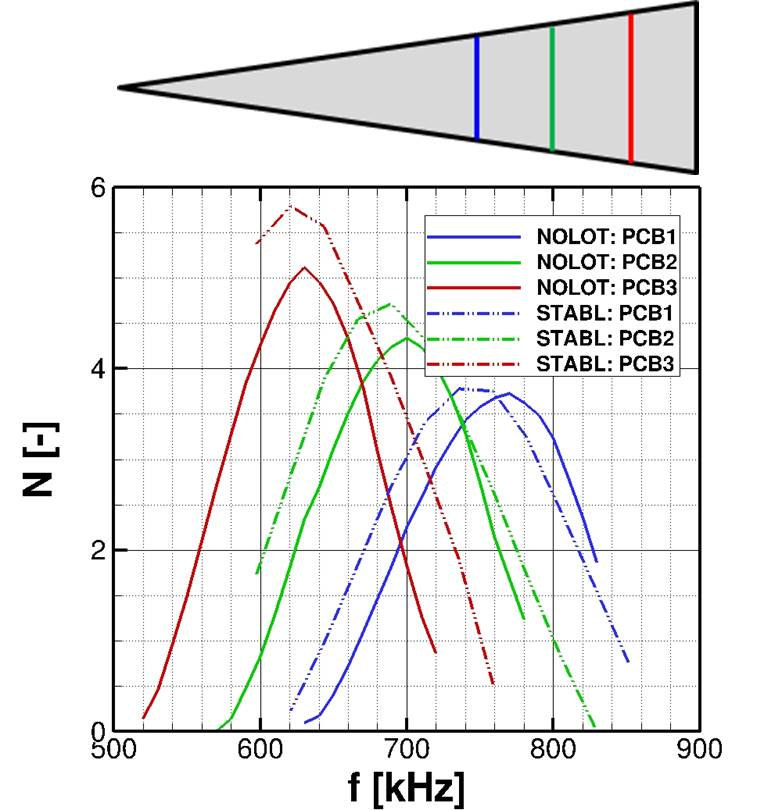
\includegraphics[width=0.6\textwidth]{pics/2018_1324_nolot_stabl_n_f.jpg}
	\caption{$N$-factor as function of the frequency - numerical results (NOLOT and STABL)}
	\label{fig:1324_n_f}
\end{figure}

The second mode is amplified in streamwise direction. Due to the increase of the boundary-layer thickness the frequencies of the distribution are shifted to lower values, which can be explained with the following relation between boundary-layer thickness $\delta$ and wavelength $\lambda$\cite{Stetson_1984, Mack_1984}\hspace{0.02cm}: $\lambda \approx 2 \hspace{0.1cm}\delta$. The calculations with NOLOT, marked by solid lines, neglected here the real gas effects (for the base flow calculations as well as the NOLOT analyses). In contrast, the base-flow calculations for STABL and the STABL calculations (dashed lines) itself include chemical effects, which results in higher amplified second modes and additional in a lightly shift of the frequency range.\\

These numerical results will be compared with the experimental measurements for all mentioned test cases of table \ref{tab:test_cases}.



\bibliographystyle{unsrtdin}
\begin{thebibliography}{33}

\bibitem {Hannemann_2008}
Hannemann, K., Martinez Schramm, J., Sebastian, K., ``Recent extensions to the High Enthalpy shock tunnel Göttingen (HEG)'', \textit{2nd International ARA Days}, Arcachon, Frankreich, 2008

\bibitem {Hein_1994}
Hein, S., Bertolotti, F. P.,  Simen, M., Hanifi, A., Henningson, D., ``Linear nonlocal instability analysis - the linear NOLOT code'',  \textit{DLR-IB}, 223-94 A56, 1994

\bibitem {Mack_1984}
Mack, L. M., ``Boundary layer linear stability theory'', \textit{AGARD Special course on stability and transition of laminar flow},  1984

\bibitem {Malik_1989}
Malik, M. R.: ``Prediction and control of transition in supersonic and hypersonic boundary layers'', \textit{AIAA Journal}, Vol. 27, No. 11, pp. 1487-1493, 1989

\bibitem {Schneider_1999}
Schneider, S., ``Flight Data for Boundary Layer Transition at Hypersonic and Supersonic Speeds'', \textit{Journal of Spacecraft and Rockets}, Vol. 36, No. 1, 1999, pp. 8-20, Rockets, Vol. 36, No. 1, 1999, pp. 8–20

\bibitem {Schneider_2004}
Schneider, S., ``Hypersonic Laminar-Turbulent Transition on Circular Cones and Scramjets Forebodies'', \textit{Process in Aerospace Sciences}, Vol. 40, No. 1-2, 2004, pp. 1-50

\bibitem {Stetson_1984}
Stetson, K. F., Thompson, E. R., Donaldson, J. C., Siler, L. G., ``Laminar boundary-layer stability experiments on a cone at Mach 8, Part 2: Blunt cone'', \textit{AIAA Paper}, AIAA84-0006, 198


\end{thebibliography}

\end{document}

% - Release $Name:  $ -